\documentclass[3p]{elsarticle} %review=doublespace preprint=single 5p=2 column
%%% Begin My package additions %%%%%%%%%%%%%%%%%%%
\usepackage[hyphens]{url}



\usepackage{lineno} % add
\providecommand{\tightlist}{%
  \setlength{\itemsep}{0pt}\setlength{\parskip}{0pt}}

\bibliographystyle{elsarticle-harv}
\biboptions{sort&compress} % For natbib
\usepackage{graphicx}
\usepackage{booktabs} % book-quality tables
%%%%%%%%%%%%%%%% end my additions to header

\usepackage[T1]{fontenc}
\usepackage{lmodern}
\usepackage{amssymb,amsmath}
\usepackage{ifxetex,ifluatex}
\usepackage{fixltx2e} % provides \textsubscript
% use upquote if available, for straight quotes in verbatim environments
\IfFileExists{upquote.sty}{\usepackage{upquote}}{}
\ifnum 0\ifxetex 1\fi\ifluatex 1\fi=0 % if pdftex
  \usepackage[utf8]{inputenc}
\else % if luatex or xelatex
  \usepackage{fontspec}
  \ifxetex
    \usepackage{xltxtra,xunicode}
  \fi
  \defaultfontfeatures{Mapping=tex-text,Scale=MatchLowercase}
  \newcommand{\euro}{€}
\fi
% use microtype if available
\IfFileExists{microtype.sty}{\usepackage{microtype}}{}
\usepackage{graphicx}
% We will generate all images so they have a width \maxwidth. This means
% that they will get their normal width if they fit onto the page, but
% are scaled down if they would overflow the margins.
\makeatletter
\def\maxwidth{\ifdim\Gin@nat@width>\linewidth\linewidth
\else\Gin@nat@width\fi}
\makeatother
\let\Oldincludegraphics\includegraphics
\renewcommand{\includegraphics}[1]{\Oldincludegraphics[width=\maxwidth]{#1}}
\ifxetex
  \usepackage[setpagesize=false, % page size defined by xetex
              unicode=false, % unicode breaks when used with xetex
              xetex]{hyperref}
\else
  \usepackage[unicode=true]{hyperref}
\fi
\hypersetup{breaklinks=true,
            bookmarks=true,
            pdfauthor={},
            pdftitle={Critical slowing down anticipates emergence and elimination of measles},
            colorlinks=false,
            urlcolor=blue,
            linkcolor=magenta,
            pdfborder={0 0 0}}
\urlstyle{same}  % don't use monospace font for urls

\setcounter{secnumdepth}{0}
% Pandoc toggle for numbering sections (defaults to be off)
\setcounter{secnumdepth}{0}
% Pandoc header

\journal{Proceedings of the Royal Society B}
\usepackage{lineno}
\linenumbers
\usepackage{mathptmx}
\renewcommand{\theaffn}{\arabic{affn}}

\begin{document}
\begin{frontmatter}

  \title{Critical slowing down anticipates emergence and elimination of measles}
    \author[UGA,CEID]{Andrew T. Tredennick\corref{c1}}
   \ead{atredenn@gmail.com} 
   \cortext[c1]{Corresponding Author}
    \author[UGA,CEID]{Eamon O'Dea}
  
  
    \author[other]{TBD}
  
  
    \author[UGA,CEID,ID]{Pejman Rohani}
  
  
    \author[UGA,CEID]{John M. Drake}
   \ead{jdrake@uga.edu} 
  
      \address[UGA]{Odum School of Ecology, University of Georgia, Athens, GA 30602, USA}
    \address[CEID]{Center for the Ecology of Infectious Diseases, University of Georgia,
Athens, GA 30602, USA}
    \address[other]{A University of Somewhere}
    \address[ID]{Department of Infectious Diseases, University of Georgia, Athens, GA
30602, USA}
  
  \begin{abstract}
  Forecasts of the emergence, re-emergence, and elimination of human
  infectious diseases would allow for proactive, rather than reactive,
  decisions that could save lives. Recent theory suggests that a generic
  feature of dynamical systems approaching a tipping point -- critical
  slowing down -- can anticipate disease emergence and elimination.
  Empirical demonstrations of critical slowing down in real disease
  dynamics are scarce, but are essential before we can implement
  model-independent outbreak detection systems. Here, we use
  empirically-based, mechanistic models of measles transmission in four
  Nigerien cities to detect critical slowing down through statistical
  early warning signals. We find that several early warning signals
  accurately anticipate measles re-emergence and elimination, suggesting
  that critical slowing down can be detected before tipping points in real
  disease dynamics. Broadly, our findings suggest that early warning
  signals, coupled with decision-support algorithms and expert judgment,
  could provide the basis for outbreak early detection systems.
  \end{abstract}
   \begin{keyword} critical slowing down, early warning signals, epidemiology, measles, infectious disease\end{keyword}
 \end{frontmatter}

\hypertarget{introduction}{%
\section{Introduction}\label{introduction}}

Forecasts of the emergence and re-emergence of infectious diseases have
the potential to save lives, money, and human productivity by allowing
for proactive, rather than reactive, preparedness measures {[}1{]}.
Similarly, indicators of the elimination of infectious diseases can
signal the effectiveness of ``end game'' strategies aimed at disease
eradication {[}2{]}. Predicting (re)emergence and elimination is
possible with complex mathematical models of disease transmission, but
their success relies on detailed understanding of the underlying
transmission dynamics and adequate data {[}3{]}. We often do not have
enough information to parameterize such models. An alternative approach
is to use model-independent statistical signals that portend infectious
disease (re)emergence and elimination by detecting critical slowing down
as the system approaches a critical transition {[}4{]}.

Emergence and elimination of an infectious disease both involve a
critical transition (technically, a \emph{transcritical bifurcation}).
The transition typically occurs at the critical point where the basic
reproduction number (\(R_0\), the number of secondary cases that arise
from a single infected case in a fully susceptible population) is equal
to one {[}5{]}. Thus, subcritical (\(R_0 < 1\)) and supercritical
(\(R_0 > 1\)) systems represent alternative modes of fluctuation
{[}4,6,7{]}.

Critical transitions in stochastic systems, such as systems of disease
transmission, are often associated with critical slowing down, a
reduction in the resilience of a system to perturbations {[}8{]}.
Critical slowing down (CSD), in turn, is associated with changes in the
dynamical features of the system: early warning signals (EWS) such as an
increase in the variance and autocorrelation {[}6,9{]}. Recent
theoretical work suggests that CSD occurs as disease dynamics approach
\(R_0 = 1\) from below (emergence) {[}4,10{]} and from above
(elimination) {[}2,4,11{]}, and that several EWS anticipate the critical
transition {[}12--14{]}. Empirical tests of EWS and associated CSD are,
however, scarce. Documenting CSD in real disease dynamics is an
essential first step toward the development of model-independent
outbreak detection systems {[}1{]}.

Here, we use empirically-based model simulations of measles dynamics to
test whether CSD anticipates critical transitions in real disease
dynamics. We focus on two scenarios: the re-emergence of measles
following a large outbreak, a situation typical of measles dynamics in
sub-Saharan Africa {[}15{]}, and the elimination of measles by a
vaccination campaign. We seek to answer two related questions. First,
can CSD distinguish between time series of disease incidence when the
underlying dynamics are far from and near to a critical transition? If
so, then CSD can anticipate disease re-emergence and elimination.
Second, how does the distance to and the rate of approaching the
threshold impact the anticipatory skill of CSD?

To answer these questions, we fit mechanistic models of disease
transmission to time series of measles incidence in four Nigerien
cities. We then use the fitted models to perform model experiments
designed to test the performance of several EWS, which quantify CSD, at
anticipating re-emergence and elimination. Our results confirm
theoretical expectations about several EWS and associated CSD. In
particular, we show that CSD before a critical transition is detectable
by several EWS in realistic scenarios, and they do so using much shorter
time series than used in theoretical studies. However, our study
highlights the limitations of EWS in situations where disease
re-emergence and elimination occurs rapidly. Moreoever, and contrary to
theoretical expectations {[}4{]}, we find that EWS perform better at
detecting CSD before re-emergence than before elimination.

\hypertarget{materials-and-methods}{%
\section{Materials and Methods}\label{materials-and-methods}}

\hypertarget{data}{%
\subsection{Data}\label{data}}

We used weekly measles case report data from four Nigerien cities:
Agadez, Maradi, Niamey, and Zinder (figure \ref{data-plot}\emph{a}). The
data were collected over an 11 year period from 1995-2005 (figure
\ref{data-plot}\emph{b}). These data are ideal for testing theory on CSD
in disease dynamics because each city has different population sizes,
has different dynamics in terms of outbreak sizes and length of
inter-epidemic periods, and each time series has different amounts of
demographic stochasticity due to differences in population size. Such
differences provide a natural gradient of ``noise'' that may influence
CSD {[}16--19{]}. The data come from {[}\emph{somewhere/someone}{]}, and
used here with permission from {[}\emph{somewhere/someone}{]}.

\begin{figure}
\centering
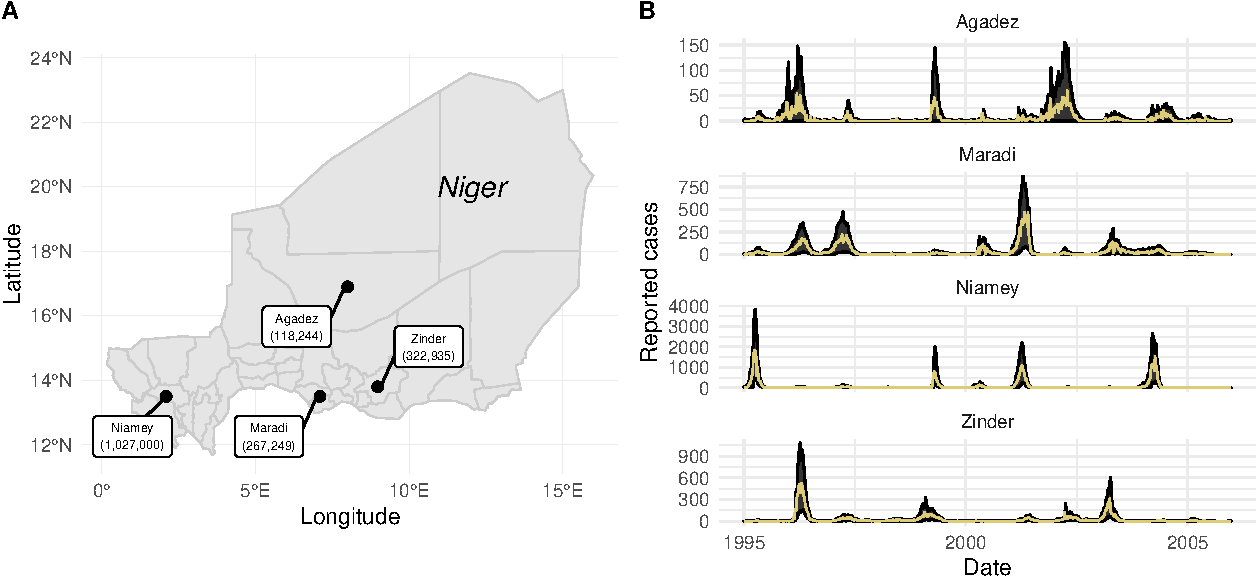
\includegraphics{measles-ews-manuscript_files/figure-latex/data-plot-1.pdf}
\caption{Locations of data sources and observed and predicted measles
dynamics. (A) Locations and population sizes (in parantheses) of our
four focal cities in Niger. (B) Time series of weekly reported cases
(yellow solid lines) and the 95\% prediction intervals (black ribbons)
for one-week-ahead predictions from our fitted SEIR models for each
city. \label{data-plot}}
\end{figure}

\hypertarget{stochastic-seir-model}{%
\subsection{\texorpdfstring{Stochastic \emph{SEIR}
model}{Stochastic SEIR model}}\label{stochastic-seir-model}}

The model is a discrete-time approximation of a continuous-time SEIR
model with limited demography, specified as a set of difference
equations,

\begin{align}
S_{t+dt} &= n_{S,t} - n_{E,t} \\
E_{t+dt} &= n_{E,t} - n_{I,t} \\
I_{t+dt} &= n_{I,t} + n_{O,t} - n_{R,t},
\end{align}

\noindent{}where \(\textbf{n}_t\) are random variables representing the
number of individuals transitioning into or out of each class at each
timestep \(t \rightarrow t+dt\). \(n_{S}\) is the number of births,
\(n_{E}\) is the number of newly infected individuals that have the
disease but are not infectious, \(n_{I}\) is the number of newly
infectious indiviuals, \(n_{O}\) is the number of imported infections,
and \(n_{R}\) is the number of newly recovered individuals who are no
longer infectious and have life-long immunity. The stochastic random
variables are specified as follows:

\begin{align}
n_{S,t} &\sim \text{Poisson}(\mu_t N_t \times dt) \\
n_{E,t} &\sim \text{Binomial}(\lambda_{E,t}, S_{t}) \\
n_{I,t} &\sim \text{Binomial}(\lambda_{I,t}, E_{t}) \\
n_{O,t} &\sim \text{Poisson}(\psi \times dt) \\
n_{R,t} &\sim \text{Binomial}(\lambda_{R,t}, I_{t}),
\end{align}

\noindent{}where \(\mu_t\) is the birth rate at time \emph{t}, \(\psi\)
is the rate of imported infections, and \(\lambda_E\), \(\lambda_I\),
and \(\lambda_R\) are the probabilities of exposure, becoming
infectious, and recovery, respectively. These probabilities reflect the
processes of tranmission, transition from the latent period to the
infectious period, and recovery, which we model as:

\begin{align}
\lambda_{E,t} &= 1 - e^{-\frac{\beta_t I_t dt}{N_t}} \\
\lambda_{I,t} &= 1 - e^{-\eta E_{t} dt} \\
\lambda_{R,t} &= 1 - e^{-\gamma I_{t} dt},
\end{align}

\noindent{}where \(\beta_t\) is time-varying rate of transmission,
\(\eta\) is time-invariant rate from the exposed class to the infectious
class, and \(\gamma\) is time-invariant recovery rate. We model rate of
transmission as:

\begin{equation}
\beta_t = \beta \left(1 + \sum^6_{i=1} q_i \xi_{i_{t}} \right) \Gamma_t.
\end{equation}

\(\beta\) is the mean transmission rate, \(\psi\) accounts for measles
infections from external sources that are not part of the local
dynamics, and the term \(\sum^6_{i=1} q_i \xi_{i_{t}}\) is a B-spline to
model seasonality in transmission. The B-spline bases (\(\xi_{i_{t}}\))
are periodic with a 1 year period. The transmission rate (\(\beta_t\))
is also subject to stochastic process noise at each time step,
\(\Gamma_t\), which we model as gamma-distributed white (temporally
uncorrelated) noise with mean 1 and variance \(\sigma^2\) {[}20{]}.

We do not include a death process in the model because the rate of
infection is much faster than the rate of death. Excluding deaths means
we can avoid making further assumptions about demographic rates -- we
are already making assumptions about birth rates (e.g., the rate is the
same across cities, but with city-specific population size). We model
demographic stochasticity in births and imported infections by drawing
time-specific values from Poisson distributions. In this model, the
effective reproduction number at time \emph{t} is:
\(R_E(t) = \frac{\beta_t}{\gamma} \frac{S_t}{N_t}\).

We assume observed case reports (\(\textbf{y}\)) are drawn from a
Negative Binomial distribution subject to a constant reporting fraction
(\(\rho\)) and dispersion parameter \(\tau\),

\begin{align}
y_t \sim \text{Negative Binomial} \left( \rho x_t, \tau \right),
\end{align}

\noindent{}where \(x_t\) are the accumulated cases that transition from
the infected class to the recovered class in a one week period.

\hypertarget{model-fitting-and-inference}{%
\subsection{Model fitting and
inference}\label{model-fitting-and-inference}}

We fit the SEIR model to time series of case reports from each of our
focal cities using Maximization by Iterated particle Filtering (MIF). We
estimated 14 parameters for each city: six seasonal transmission
parameters (\(q_i\)), mean transmission rate (\(\beta\)), three initial
conditions \(\left(S_{(t=0)},E_{(t=0)},I_{(t=0)}\right)\), the number of
imported infections (\(\psi\)), reporting fraction (\(\rho\)), one
parameter accounting for process noise (\(\sigma\)), and one parameter
accounting for measurement noise (\(\tau\)). To ensure identifiability,
and to make the model easier to fit, we assumed the infectious period
was fixed at \(1/\eta = 8\) days and the recovery period was fixed at
\(1/\gamma = 5\) days. The birth rate (\(\mu_t\)) was multiplied by 0.3
to account for the reported 70\% vaccination coverage {[}15{]}.

MIF relies on particle filtering, which estimates the likelihood of
fixed parameters by integrating state variables of a stochastic system.
To narrow in on the maximum likelihood estimates, MIF lets parameters
take a random walk during the filtering process and selectively
propagates forward parameter sets (i.e., particles) with the highest
likelihood. The variance of the random walk decreases at each iteration
of MIF, where a MIF iteration means one filtering pass through the time
series. This procedure converges toward the maximimum likelihood
estimates (MLEs), in theory.

We used the IF2 algorithm {[}21{]} implemented in the R {[}22{]} package
\texttt{pomp} {[}23,24{]} to conduct the MIF procedure. To initialize
MIF, we generated 5000 parameter sets using Latin Hypercube Sampling
over large ranges of the parameter values. We then performed two rounds
of MIF, each for 100 iterations, with 10000 particles, and geometric
cooling. For the first round of MIF we set
\texttt{cooling.facter\ =\ 1}. For the second round, which was
initialized using the collection of parameter sets from the end of the
first round, we set \texttt{cooling.factor\ =\ 0.9}. We computed the log
likelihood of 5000 final MIF parameter sets (i.e., parameter sets
collected after 200 MIF iterations) as the log of the mean likelihoods
of 50 replicate particle filters with 10000 particles each. At this
stage, we assume the parameter set with highest log likelihood is the
MLE.

We used a bootstrapping approach to estimate approximate 95\% confidence
intervals for all parameters. The procedure, which was conducted for
each city independently, is as follows. First, we simulated 100
realizations from the fitted model using the MLE parameters. Second, we
fitted the SEIR model to each of the 100 bootstrap simulations using the
same MIF procedure described above, except we initiated the parameter
search from 50 parameter sets rather then 5000. We reduced the number of
parameter sets due to the computational constraints of fitting 100
simulated data sets for each of the four cities. Third, we identified
the MLE parameter set for each of the 100 bootstrap simulations from
among the 50 MIF paramete sets. Last, we calculated summary statistics
(mean, median, quantiles) from the distribution of 100 MLE parameters
(SI text).

\hypertarget{model-assessment}{%
\subsection{Model assessment}\label{model-assessment}}

We used the MLE parameter sets to make one-week-ahead predictions and
compared observed and expected case counts. To make one-week-ahead
predictions, we used particle filtering with 50000 particles and
retained the mean and standard deviation of all latent states across all
particles before they were filtered at each time step. We used the mean
predictions (\(\mathbb{E}(\text{cases}_t)\)) to assess model fit using a
generalized coefficient of determination, calculated as:
\(R^2 = 1 - \frac{\sum_t [\mathbb{E}(\text{cases}_t) - \text{cases}_t]^2}{\sum_t [\text{mean(cases)}-\text{cases}_t]^2}\)
{[}25{]}. In addition to comparing model expectations to in-sample
observed data, we also compared our fitted SEIR models to two
benchmarking models: a negative binomial sampling model that assumes
identical and independently distributed observations and a seasonal
moving average model (SI text). We fit the benchmarking models to the
observed data and then compared models using Akaike's Information
Criterion (AIC) to account for differences in the number of model
parameters {[}26{]}.

\hypertarget{simulating-re-emergence}{%
\subsection{Simulating re-emergence}\label{simulating-re-emergence}}

To simulate re-emergence of measles, we manipulated the initial size of
the susceptible pool to simulate an increase from low \(R_E(t)\) to high
\(R_E(t)\). Doing so allows us to test whether EWS can distinguish
between windows of time when \(R_E(t)\) is far from a critical
transition and when \(R_E(t)\) is near a critical transition. We reduced
the initial fraction of susceptible individuals by multplying the MLE
for \(S_{(t=0)}\) by six discounting factors: 1e-4, 0.1, 0.2, 0.3, 0.4,
and 0.5. These discounting factors represent situations of susceptible
depletion after outbreaks of various size. After defining \(S_{(t=0)}\)
based on the discounting factor, we then set the initial number of
recovered individuals to \(R_{(t=0)} = N - S_{(t=0)}\) and set the
initial number of exposed and infected individuals to zero. Population
size, \emph{N}, was set to the mean population size for each city over
the 1995-2005 time period. We then simulated the model forward for forty
years using mean birth rate for the entire country (\(\mu = 0.05\)) and
setting the death rate equal to the birth rate (\(\mu = \nu = 0.05\)) to
achieve a constant eqiulibrium total population size over the course of
the simulation (total population size does vary, though, because of
stochasticity in the model). Forty years was long enough for \(R_E(t)\)
to reach or exceed 1 for each city. Because the model is stochastic, we
repeated these simulations 500 times for each city-susceptible discount
combination.

Next, we split each simulated time series into null and test intervals.
First, averaging across all simulations for a city-susceptible discount
combination, we found the simulation year in which \(R_E(t)\) reaches or
exceeds 1 and excluded years past that year (SI text). We split the
remaining time series into two windows of equal length (figure
\ref{emerge-aucs}\emph{a}). The null interval is the first window, where
\(R_E(t)\) is increasing but far from 1. The test interval is the second
window, where \(R_E(t)\) is increasing and approaching 1. We did this
for each city and for each level of susceptible depletion. We calculated
EWS over null and test intervals separately.

\hypertarget{simulating-elimination}{%
\subsection{Simulating elimination}\label{simulating-elimination}}

To simulate elimination, we simulated a vaccine campaign in which
vaccination coverage linearly increased over time to eventually reach
100\%, i.e.~eradication (figure S3). We ran simulations for 100 years,
starting with 50 years of dynamics at the baseline vaccine coverage
reported for Niger of 70\%, \(p = 0.7\) {[}15{]}. Note that vaccination
coverage is included in our model by discounting the birth rate of
susceptibles by \(1-p\). At year 50, we initiated the vaccination
campaign and let the model run for another 50 years. We ran simulations
across six vaccination ``speeds'' (the rate at which
\(p \rightarrow 1\); SI text), simulating situations of slow and fast
approaches to elimination. As in the re-emergence simulations, we set
the birth rate equal to the death rate to achieve a constant equilibrium
population size.

We then split each time series into null and test intervals for
calculating EWS. We define the test interval as the window of time
between the start of the vaccination campaign (year 50) and the time at
which vaccination coverage reached the vaccination threshold of
\(1 - 1/R_0\) (figure \ref{elim-aucs}\emph{a}). \(R_0\) was calculated
for each city using the MLE parameters as:
\(R_0 = \left[\eta \beta \right]/ \left[\left(\eta+\nu\right)\left(\gamma+\nu\right)\right]\),
where \(\beta\) is the maximum seasonal transmission rate. We define the
null interval as the window of time that ends at the start of the
vaccination campaign (year 49) and starts at a time that results in an
interval equal in length the test interval (figure
\ref{elim-aucs}\emph{a}). EWS were then calculated for each interval.

\hypertarget{calculating-early-warning-signals}{%
\subsection{Calculating early warning
signals}\label{calculating-early-warning-signals}}

We considered nine candidate early warning signals (Table S1). We used
the \texttt{spaero::get\_stats()} function {[}27{]} in R {[}22{]} to
calculate EWS according to the formulas in Table S1. All EWS except the
coefficient of variation are expected to increase as \(R_E(t)\)
approaches 1 from below {[}4,11,13{]}. Less is known about the behavior
of EWS as \(R_E(t)\) approaches 1 from above. But, theory does tell us
that, for SIR models, the mean should decrease, autocorrelation should
increase, and the variance should decrease {[}4{]}.

For each simulation of re-emergence and elimination, we calculated EWS
for the time series of expected cases in the null and test intervals.
This yielded a distribution of EWS over the 500 null and test intervals.
We assessed the performance of each EWS using the Area Under the Curve
(AUC) statistic. Specifically, we use AUC to calculate the amount of
overlap between the distributions of each EWS from the null and test
intervals. Values of AUC far from 0.5 (i.e., close to 0 or 1) indicate a
greater degree of separation and thus better performance of a particular
EWS in terms of classifying whether \(R_E(t)\) is close to a critical
transition. We calculated AUC as:
\(\text{AUC} = \left[r_{\text{test}} - \left(n_{\text{test}}+1\right)/2\right] / \left(n_{\text{test}}n_{\text{null}}\right)\)
where \(r_{\text{test}}\) is the sum of the ranks of test set EWS
statistics in a combined set of null and test statistics (lower numbers
have lower ranks), \(n_{\text{test}}\) is the number of test of
statistics and \(n_{\text{null}}\) is the number of null statistics. The
AUC of an EWS is the probability that a randomly chosen EWS value from
the test set is higher than an EWS value randomly chosen from the null
set {[}28{]}. Therefore, AUC should be high (closer to 1) when an EWS is
expected to increase as a critical transition is approached, whereas AUC
should be low (closer to 0) when an EWS is expected to decrease.

\begin{figure}
\centering
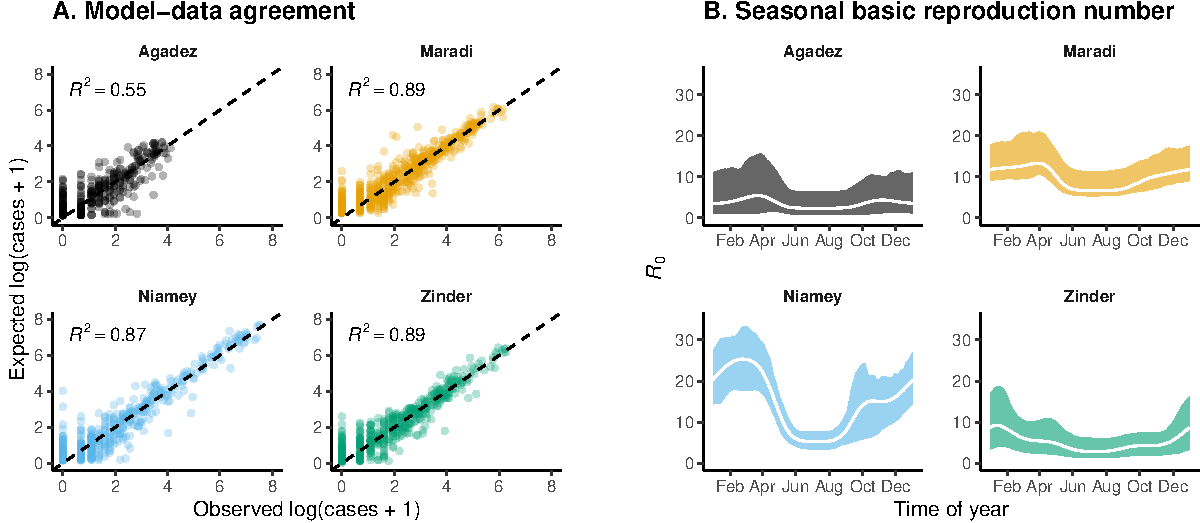
\includegraphics{measles-ews-manuscript_files/figure-latex/scatters-r0-1.pdf}
\caption{Accuracy of the fitted \emph{SEIR} models and estimated
seasonality. (A) Comparison of in-sample model predictions and
observations for each city. Expected cases are one-week-ahead
predictions from the fitted models. The dashed line shows 1:1.
Coefficients of determination (\(R^2\)) were calculated as the reduction
in the sum-of-squared errors from model predictions relative to a null
model of the mean number of cases (SI text). (B) The estimated
seasonality of the basic reproductive ratio (\(R_0\)) for each city.
\(R_0\) was calculated as:
\(\frac{\eta \beta_t}{(\eta+\nu)(\gamma+\nu)}\), where \(1/\eta\) is the
infectious period, \(1/\gamma\) is the recovery period, \(\beta_t\) is
the time-specific rate of transmission, and \(\nu\) is the death rate.
Only \(\beta_t\) is estimated by our model. We set \(1/\eta\) = 8 days,
\(1/\gamma\) = 5 days, and \(\mu = \nu\) = 0.05 for calculating \(R_0\)
as shown in this figure. The white line is \(R_0\) calculated using the
MLE parameters; shaded regions are the bootstrapped 95\% confidence
intervals. \label{scatters}}
\end{figure}

\hypertarget{results}{%
\section{Results}\label{results}}

The fitted models adequately reproduce observed dynamics (figure
\ref{data-plot}\emph{b}), with in-sample \(R^2\)s from one-week-ahead
predictions ranging from 0.54 for Agadez to 0.89 for Maradi (figure
\ref{scatters}\emph{a}). The fitted models also had lower AIC values
than two benchmarking models (SI Table Sx). Stochastic simulations of
the models displayed dynamics typical of each city (figure S1),
including the decline in seasonality amplitude as population size
decreases (figure \ref{scatters}\emph{b}) {[}15{]}. Our model for Agadez
performs poorly relative to the other cities. Maximum likelihood
estimates and bootstrapped 95\% confidence intervals for all parameters
are in the SI text (Tables Sx-Sz).

On the approach to re-emergence the EWS generally perform as expected by
theory. Most EWS increased as the critical transition is approached,
resulting in positive AUC values near 1 (figure \ref{emerge-aucs}).
Skewness, kurtosis, and coefficient of variation performed poorly across
all levels of susceptible depletion in all cities. Thus, these metrics
are unreliable.

Variance, mean, index of dispersion, decay time, autocovariance, and
autocorrelation all perform equally well at predicting re-emergence
(figure \ref{emerge-aucs}\emph{c}). Their performance declines as the
amount of susceptible depletion decreases. This is expected because more
rapid returns to \(R_E(t)=1\) result in shorter null and test intervals,
making estimates of EWS less precise {[}12{]}. Moreover, as the time to
reach \(R_E(t)=1\) decreases, the chance of a bifurcation delay
increases because of the changing equilibrium of \(R_0\) combined with
demographic stochasticity {[}10,12{]}. Thus, re-emergence may prove
difficult to anticipate in ``fast'' transmission systems, as
demonstrated theoretically by {[}12{]} and seen here when susceptible
depletion was relatively small (figure \ref{emerge-aucs}\emph{c}).

\begin{figure}
\centering
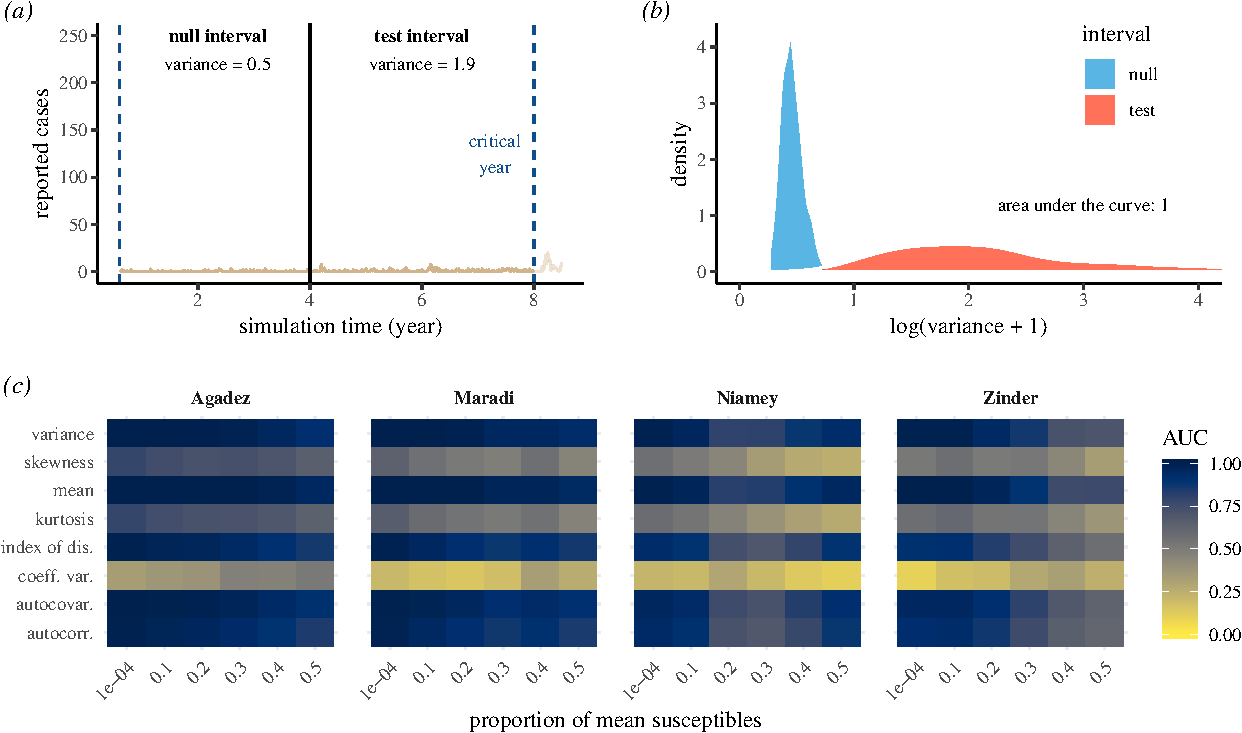
\includegraphics{measles-ews-manuscript_files/figure-latex/emergence-results-1.pdf}
\caption{Performance of early warning signals (EWS) over fixed windows
on the approach to emergence. (A) A typical example of an emergence
simulation for Maradi. The two vertical blue lines indicate the start
(left-most line) and end (line for critical year) of the full window.
The black line demarcates the division between the equal-length null and
test intervals, in which we show the calculated variance. (B) Empirical
densities of variance in the null and test intervals across 500
simulations and the associated area under the curve (AUC) statistic. (C)
Heatmap of AUC statistics for each EWS at each level of susceptible
discount factor. AUC values closer to 0 or 1 indicate higher ability to
distinguish among time series near and far from a critical transition.
See Fig. Sx for visualization of how susceptible discounting factor maps
to number of weeks in the null and test intervals. \label{emerge-aucs}}
\end{figure}

The EWS did not perform as well when anticipating elimination, relative
to emergence (figure \ref{elim-aucs}). Only three metrics are reliable:
mean, autocovariance, and variance. All three metrics decreased as
\(R_E(t)\) approached the critical transition (figure S5). As in the
case of anticipating elimination, AUC values decreased as the speed of
the vaccine campaign increased (figure \ref{elim-aucs}\emph{c}). Again,
this is because of shorter null and test intervals.

\begin{figure}
\centering
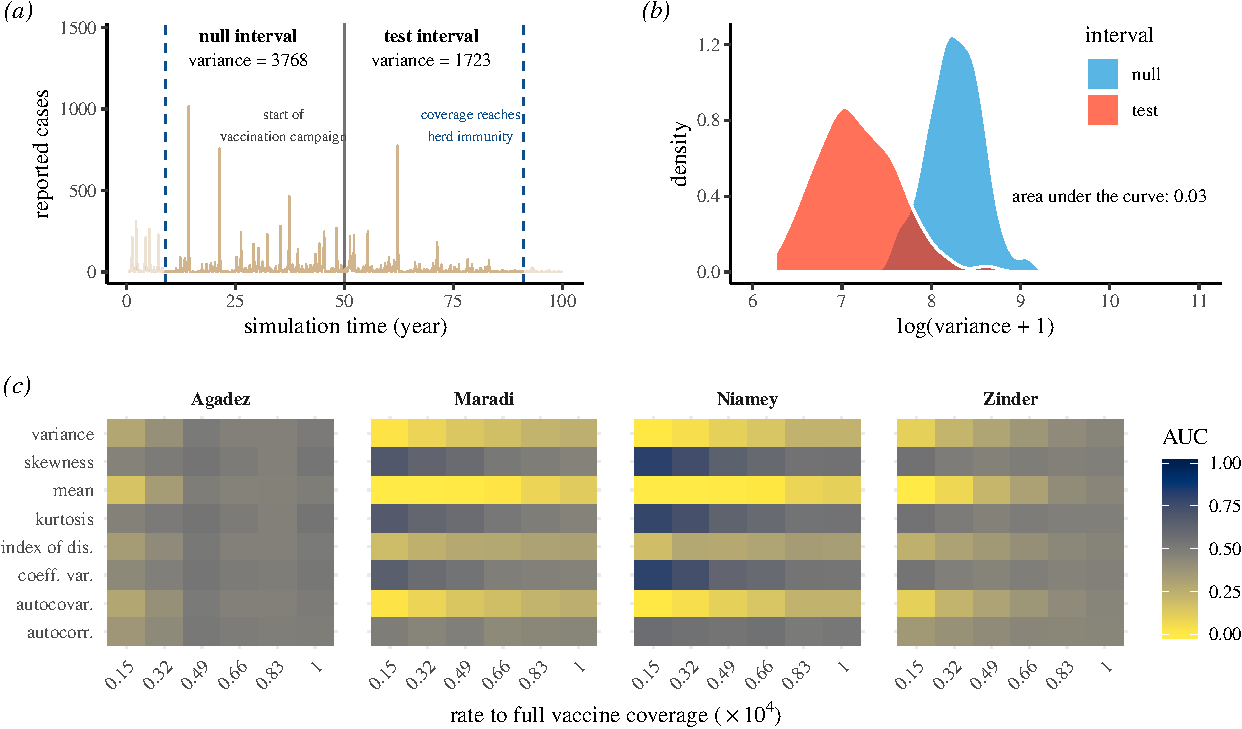
\includegraphics{measles-ews-manuscript_files/figure-latex/elimination-1.pdf}
\caption{Performance of early warning signals (EWS) over fixed windows
on the approach to elimination. (A) A typical example of an elimination
simulation for Maradi. The two vertical blue lines indicate the start
(left-most line) and end (line for critical year) of the full window.
The black line demarcates the division between the equal-length null and
test intervals, in which we show the calculated variance. (B) Empirical
densities of variance in the null and test intervals across 500
simulations and the associated area under the curve (AUC) statistic. (C)
Heatmap of AUC statistics for each EWS at each speed of approach to herd
immunity. AUC values closer to 0 or 1 indicate higher ability to
distinguish among time series near and far from a critical transition.
See Fig. Sx for visualization of how vaccination speed maps to number of
weeks in the null and test intervals. \label{elim-aucs}}
\end{figure}

In all, the suite of EWS suggest that critical slowing down does occur
in measles dynamics as a critical transition is approached. We found
similar results for the approach to elimination when calculating EWS
over a moving window of 35 weeks in the null and test intervals (SI
text, figure S7). But, all EWS performed worse when predicting the
approach to emergence over the moving window (figure S7).

\hypertarget{discussion}{%
\section{Discussion}\label{discussion}}

Using empirically-based disease transmission models, we found evidence
of critical slowing down before critical transitions to re-emergence and
elimination of measles. This evidence comes from the fact that several
EWS accurately anticipate the critical transition.

A potential limitation of our findings is that the levels of susceptible
depletion we modeled (figure \ref{emerge-aucs}C) might be lower than the
levels that occur in reality. To check the relevance of this limitation,
we calculated the level of susceptible depletion after outbreaks
(defined as years where the total number of cases reached 80\% of the
maximum observed) across one hundred replicate simulations (SI text). We
found that susceptible depletion was less than 0.5, the smallest
susceptible depletion level we tested, for 0.9\% of outbreaks in Agadez,
21\% of outbreaks in Maradi, 100\% of outbreaks in Niamey, and 26\% of
outbreaks in Zinder. These statistics do not detract from our main
findings of CSD in measles dynamics, but they do suggest that EWS might
be less useful in some cases than in others. For example, AUC values for
emergence at the 0.5 level of susceptible depletion are already low for
most cities (figure \ref{aucs}A). Thus, EWS are not practical for cities
that rarely experience levels of susceptible depletion below 0.5 (e.g.,
Agadez).

Our results should encourage efforts to develop model-independent early
warning systems for infectious diseases {[}1{]}. We have shown that
critical slowing down precedes tipping points in real disease dynamics,
but how to operationalize the phenomenon of critical slowing down
remains an open research area {[}29{]}. Emerging technologies like
artifical intelligence might offer new ways to find optimal detection
thresholds for early warning signals. But there will always be a role
for expert judgement. Early warning signals, though powerful and now
accompanied with empirical support, will likely be just one part of a
decision-support toolkit.

\hypertarget{acknowledgments}{%
\section{Acknowledgments}\label{acknowledgments}}

This research was funded by the National Institute of General Medical
Sciences of the National Institutes of Health (Award Number
U01GM110744). The funders had no role in study design, data collection
and analysis, decision to publish, or preparation of the manuscript.
This work was done on the Olympus High Performance Compute Cluster
located at the Pittsburgh Supercomputing Center at Carnegie Mellon
University, which is supported by National Institute of General Medical
Sciences Modeling Infectious Disease Agent Study (MIDAS) Informatics
Services Group grant 1U24GM110707.

\hypertarget{references}{%
\section*{References}\label{references}}
\addcontentsline{toc}{section}{References}

\hypertarget{refs}{}
\leavevmode\hypertarget{ref-Han2016}{}%
1. Han BA, Drake JM. 2016 Future directions in analytics for infectious
disease intelligence. \emph{EMBO reports}, e201642534.
(doi:\href{https://doi.org/10.15252/embr.201642534}{10.15252/embr.201642534})

\leavevmode\hypertarget{ref-Drake2017}{}%
2. Drake JM, Hay SI. 2017 Monitoring the path to the elimination of
infectious diseaes. \emph{Tropical Medicine and Infectious Disease}
\textbf{2}, 20.

\leavevmode\hypertarget{ref-Metcalf2017}{}%
3. Metcalf CJE, Lessler J. 2017 Opportunities and challenges in modeling
emerging infectious diseases. \emph{Science} \textbf{357}, 149--152.
(doi:\href{https://doi.org/10.1126/science.aam8335}{10.1126/science.aam8335})

\leavevmode\hypertarget{ref-ORegan2013}{}%
4. O'Regan SM, Drake JM. 2013 Theory of early warning signals of disease
emergenceand leading indicators of elimination. \emph{Theoretical
Ecology} \textbf{6}, 333--357.
(doi:\href{https://doi.org/10.1007/s12080-013-0185-5}{10.1007/s12080-013-0185-5})

\leavevmode\hypertarget{ref-Heffernan2005}{}%
5. Heffernan JM, Smith RJ, Wahl LM. 2005 Perspectives on the basic
reproductive ratio. \emph{Journal of the Royal Society Interface}
\textbf{2}, 281--293.
(doi:\href{https://doi.org/10.1098/rsif.2005.0042}{10.1098/rsif.2005.0042})

\leavevmode\hypertarget{ref-Scheffer2009}{}%
6. Scheffer M \emph{et al.} 2009 Early-warning signals for critical
transitions. \emph{Nature} \textbf{461}, 53--59.
(doi:\href{https://doi.org/10.1038/nature08227}{10.1038/nature08227})

\leavevmode\hypertarget{ref-Scheffer2012}{}%
7. Scheffer M \emph{et al.} 2012 Anticipating critical transitions.
\emph{Science} \textbf{338}, 344--348.
(doi:\href{https://doi.org/10.1126/science.1225244}{10.1126/science.1225244})

\leavevmode\hypertarget{ref-VanNes2007}{}%
8. Nes EH van, Scheffer M. 2007 Slow Recovery from Perturbations as a
Generic Indicator of a Nearby Catastrophic Shift. \emph{The American
Naturalist} \textbf{169}, 738--747.
(doi:\href{https://doi.org/10.1086/516845}{10.1086/516845})

\leavevmode\hypertarget{ref-Carpenter2006}{}%
9. Carpenter SR, Brock WA. 2006 Rising variance: A leading indicator of
ecological transition. \emph{Ecology Letters} \textbf{9}, 311--318.
(doi:\href{https://doi.org/10.1111/j.1461-0248.2005.00877.x}{10.1111/j.1461-0248.2005.00877.x})

\leavevmode\hypertarget{ref-Dibble2016}{}%
10. Dibble CJ, O'Dea EB, Park AW, Drake JM. 2016 Waiting time to
infectious disease emergence. \emph{Journal of the Royal Society
Interface} \textbf{13}, 20160540.
(doi:\href{https://doi.org/10.1098/rsif.2016.0540}{10.1098/rsif.2016.0540})

\leavevmode\hypertarget{ref-ORegan2016}{}%
11. O'Regan SM, Lillie JW, Drake JM. 2016 Leading indicators of
mosquito-borne disease elimination. \emph{Theoretical Ecology}
\textbf{9}, 269--286.
(doi:\href{https://doi.org/10.1007/s12080-015-0285-5}{10.1007/s12080-015-0285-5})

\leavevmode\hypertarget{ref-Brett2017}{}%
12. Brett TS, Drake JM, Rohani P. 2017 Anticipating the emergence of
infectious diseases. \emph{Journal of the Royal Society Interface}
\textbf{14}, 20170115.
(doi:\href{https://doi.org/10.1098/rsif.2017.0115}{10.1098/rsif.2017.0115})

\leavevmode\hypertarget{ref-Brett2018}{}%
13. Brett TS, O'Dea EB, Marty É, Miller PB, Park AW, Drake JM, Rohani P.
2018 Anticipating epidemic transitions with imperfect data. \emph{PLoS
Computational Biology} \textbf{14}, e1006204.
(doi:\href{https://doi.org/10.1371/journal.pcbi.1006204}{10.1371/journal.pcbi.1006204})

\leavevmode\hypertarget{ref-Miller2017}{}%
14. Miller PB, O'Dea EB, Rohani P, Drake JM. 2017 Forecasting infectious
disease emergence subject to seasonal forcing. \emph{Theoretical Biology
and Medical Modelling} \textbf{14}, 17.
(doi:\href{https://doi.org/10.1186/s12976-017-0063-8}{10.1186/s12976-017-0063-8})

\leavevmode\hypertarget{ref-Ferrari2008}{}%
15. Ferrari MJ, Grais RF, Bharti N, Conlan AJ, Bjørnstad ON, Wolfson LJ,
Guerin PJ, Djibo A, Grenfell BT. 2008 The dynamics of measles in
sub-Saharan Africa. \emph{Nature} \textbf{451}, 679--684.
(doi:\href{https://doi.org/10.1038/nature06509}{10.1038/nature06509})

\leavevmode\hypertarget{ref-Hastings2010}{}%
16. Hastings A, Wysham DB. 2010 Regime shifts in ecological systems can
occur with no warning. \emph{Ecology Letters} \textbf{13}, 464--472.
(doi:\href{https://doi.org/10.1111/j.1461-0248.2010.01439.x}{10.1111/j.1461-0248.2010.01439.x})

\leavevmode\hypertarget{ref-Dakos2012a}{}%
17. Dakos V, Van Nes EH, D'Odorico P, Scheffer M. 2012 Robustness of
variance and autocorrelation as indicators of critical slowing down.
\emph{Ecology} \textbf{93}, 264--271.
(doi:\href{https://doi.org/10.1890/11-0889.1}{10.1890/11-0889.1})

\leavevmode\hypertarget{ref-ODea2018a}{}%
18. O'Dea EB, Park AW, Drake JM. 2018 Estimating the distance to an
epidemic threshold. \emph{Journal of the Royal Society Interface}
\textbf{15}, 20180034.
(doi:\href{https://doi.org/10.1098/rsif.2018.0034}{10.1098/rsif.2018.0034})

\leavevmode\hypertarget{ref-ORegan2018}{}%
19. O'Regan SM, Burton DL. 2018 How Stochasticity Influences Leading
Indicators of Critical Transitions. \emph{Bulletin of Mathematical
Biology} \textbf{80}, 1630--1654.
(doi:\href{https://doi.org/10.1007/s11538-018-0429-z}{10.1007/s11538-018-0429-z})

\leavevmode\hypertarget{ref-Breto2011}{}%
20. Bretó C, Ionides EL. 2011 Compound Markov counting processes and
their applications to modeling infinitesimally over-dispersed systems.
\emph{Stochastic Processes and their Applications} \textbf{121},
2571--2591.
(doi:\href{https://doi.org/10.1016/j.spa.2011.07.005}{10.1016/j.spa.2011.07.005})

\leavevmode\hypertarget{ref-Ionides2015}{}%
21. Ionides EL, Nguyen D, Atchadé Y, Stoev S, King AA. 2015 Inference
for dynamic and latent variable models via iterated, perturbed Bayes
maps. \emph{Proceedings of the National Academy of Sciences}
\textbf{112}, 719--724.
(doi:\href{https://doi.org/10.1073/pnas.1410597112}{10.1073/pnas.1410597112})

\leavevmode\hypertarget{ref-R2017}{}%
22. R Core Team. 2017 R: A language and environment for statistical
computing.

\leavevmode\hypertarget{ref-King2016}{}%
23. King AA, Nguyen D, Ionides EL. 2016 Statistical Inference for
Partially Observed Markov Processes via the R Package pomp.
\emph{Journal Of Statistical Software} \textbf{69}, 1--43.
(doi:\href{https://doi.org/10.18637/jss.v069.i12}{10.18637/jss.v069.i12})

\leavevmode\hypertarget{ref-King2018}{}%
24. King AA \emph{et al.} 2018 pomp: Statistical Inference for Partially
Observed Markov Processes (R package, version 1.18).

\leavevmode\hypertarget{ref-Martinez-Bakker2015}{}%
25. Martinez-Bakker M, King AA, Rohani P. 2015 Unraveling the
transmission ecology of polio. \emph{PLoS Biology}
(doi:\href{https://doi.org/10.1371/journal.pbio.1002172}{10.1371/journal.pbio.1002172})

\leavevmode\hypertarget{ref-Akaike1973}{}%
26. Akaike H. 1973 Information theory and an extension of the maximum
likelihood princilple. In \emph{Proceedings of the 2nd international
symposium on information theory}, pp. 267--281.
(doi:\href{https://doi.org/10.1007/978-0-387-98135-2}{10.1007/978-0-387-98135-2})

\leavevmode\hypertarget{ref-ODea2018}{}%
27. O'Dea EB. 2018 spaero: Software for Project AERO (R package version
0.3.0).

\leavevmode\hypertarget{ref-Fawcett2006}{}%
28. Fawcett T. 2006 An introduction to ROC analysis. \emph{Pattern
Recognition Letters} \textbf{27}, 861--874.
(doi:\href{https://doi.org/https://doi.org/10.1016/j.patrec.2005.10.010}{https://doi.org/10.1016/j.patrec.2005.10.010})

\leavevmode\hypertarget{ref-Shmueli2010}{}%
29. Shmueli G, Burkom H. 2010 Statistical challenges facing early
outbreak detection in biosurveillance. \emph{Technometrics} \textbf{52},
39--51.
(doi:\href{https://doi.org/10.1198/TECH.2010.06134}{10.1198/TECH.2010.06134})

\end{document}


